\documentclass{ualrdissertation}

% Document Options:
%
% Note if you want to save paper when printing drafts,
% replace the above line by
%
%   \documentclass[draft]{iitthesis}
%
% See Help file for more about options.
\usepackage{graphicx}  % Written by David Carlisle and Sebastian Rahtz

\newtheorem{theorem}{Theorem}
\newtheorem{lemma}{Lemma}
\newtheorem{corollary}{Corollary}
\newtheorem{definition}{Definition}
\newtheorem{example}{Example}
\newtheorem{property}{Property}
\newtheorem{proposition}{Proposition}
\newtheorem{assertion}{Assertion}
\newtheorem{observation}{Observation}

\usepackage{float}

\usepackage{enumerate}
\usepackage{booktabs}
\usepackage{cite}
\usepackage{url}
\usepackage{xcolor}
\usepackage{blindtext}

\usepackage{pifont}

\usepackage{adjustbox}
\usepackage{array}

% Packages are explained in the Help document.
%\raggedbottom
%this is intent to kill the widows and orphans...
%A new paragraph begun at the bottom of a page must have at least two
%full lines of type before a page break occurs. If too little room remains
%at the bottom of the page to accommodate two lines, the entire
%paragraph must begin on the following page. The preceding page may
%be shorter to allow for this adjustment.
%A paragraph ended at the top of a page must have at least two full
%lines of type. The preceding page may be shorter to allow for this
%adjustment.
\widowpenalty=10000
\clubpenalty=10000

\begin{document}

\bstctlcite{UALR-DISSERTATION:BSTcontrol}

%%% Declarations for Title Page %%%
\title{The VDEN: AN AFFORDABLE IPT DESIGNED FOR CONFERENCES}
\nsptitle{The VDEN: AN AFFORDABLE IPT DESIGNED FOR CONFERENCES}
\ctitle{The VDEN: AN AFFORDABLE IPT DESIGNED FOR CONFERENCES}

\author{Alexander Jaeger}
\degree{Master of Science}
\program{Information Science}
\dept{Information Science}
\college{Donaghey College of Engineering and Information Technology}
\date{December 2019}
\uyear{2019}
\ms{}
\bs{B.S., University of Arkansas at Little Rock, 2016}

\adviser{Carolina Cruz-Neira}
\adviserpos{\prof{Computer Science}}

\readerone{Dirk Reiners}
\readeronepos{\prof{Information Science}}

\readertwo{Jan Springer}
\readertwopos{\prof{Computer Science}}

\coordinator{Jhon R. Talburt}
\coordinatorpos{\prof{Information Science}}

\dean{Lawrence Whitman}
\deanpos{Dean}

\copyrightnoticetrue      % crate copyright page or not
%\coadvisortrue           % add co-advisor. activate it by removing % symbol to add co-advisor

\maketitle                % create title and copyright pages

\signaturepage

%\fairusepage
%\prelimpages         % Settings of preliminary pages are done with \prelimpages command

%%% Abstract %%%
\begin{abstract}
\par \blindtext[1]

\end{abstract}



%%%  Acknowledgement %%%
\begin{acknowledgement}     % acknowledgement environment, this is optional
\par \blindtext[3]
\end{acknowledgement}


% Table of Contents
\tableofcontents
\clearpage

% List of Tables
\listoftables
\clearpage

%List of Figures
\listoffigures
\clearpage


% \clearpage

\textpages     % Settings of text-pages are done with \textpages command

\Chapter{Introduction}
\blindtext[1]

\clearpage


\Chapter{Generalized Design of a CAVE System}\label{chapter:standardCAVEChapter}

%\Section[The MiniCAVE: A Voice Controlled IPT Environment]{
%	\textit{The MiniCAVE: A Voice Controlled IPT Environment} 
%	\newline By Edward Wegman Et Al \hfill 1999
%}

\filbreak
\Section[Display Technology]{Display Technology} \\

\filbreak
\noindent\textbf{Monitors}\\

\filbreak
\noindent LCD\\

\filbreak
\noindent LED\\

\filbreak
\noindent\textbf{Projectors}\\


\filbreak
\noindent LCD\\


\filbreak
\noindent DLP\\


\filbreak
\Section[Computing]{Computing}

A CAVE system requires rendering one image per eye on the screen. Robert Belleman et Al specifies a variety of computing configurations to support a CAVE \cite{belleman}.

\filbreak
\noindent\textbf{One Hosts with Two Graphics Adapters}\\
\textcolor{red}{!!! - Warning! Not sure about this}
\begin{center}
	\textcolor{blue}{Image of One Host with Two Graphics Adapters}
\end{center}

With one set of CPUs controlling a handful of graphics systems, we can support multi-display rendering. In the 20th century, SGI machines were modeled with this architecture and the  21st century saw consumer PCs becoming equipped to handle multiple graphics cards. 

The overarching problem is that consumer PCs typically support at most 2 graphics cards. CAVEs require at minimum of 4 displays, thus two cards that can handle two displays each would be suitable. Robert Belleman et Al notes that in 2001 these PCs could not be built due to the limitations in the number of AGP slots \cite{belleman}.

\filbreak
\noindent\textbf{Two Hosts with Two Graphics Adapters}\\
\begin{center}
	\textcolor{blue}{Image of Two Hosts with Two Graphics Adapters}
\end{center}

By splitting the responsibility of rendering across two computers, the rendering can be done in parallel achieving better performance. 

However special precaution needs to be in place due to possible synchronization issues. These two computers are connected over a network and in theory they just have to render the scene for the given MVP matrix. However in practice, one of these computers is used to compute both eye matrices and will introduce a load imbalance. By running the matrix calculation on a third computer, we can solve the synchronization issues however the overall network traffic is doubled because we need to send both eye MVP matrices over the wire \cite{belleman}.

\filbreak
\noindent\textbf{One Host with Multi-headed Graphics Adapters}\\
\begin{center}
	\textcolor{blue}{Image of One Hosts with Multi-headed Graphics Adapters}
\end{center}

In 2001, there some support for multiple displays using a single graphics card and little support for hardware accelerated OpenGL \cite{belleman}.  By 2017, the latest Nvidia cards can support 4 displays in sync with accelerated OpenGL. This performance improvement provides consumer PCs the power to run games and simulations on multiple displays.


\filbreak
\Section[Projection]{Projection}
\begin{center}
	\textcolor{blue}{Image of Rear Projection vs Front Projection}
\end{center}


\filbreak
\Section[Stereoscopy]{Stereoscopy}

\filbreak
\noindent\textbf{Passive Stereo}\\

\filbreak
\noindent\textbf{Active Stereo}\\

\filbreak
\Section[Tracking Techniques]{Tracking Techniques}

\clearpage

\Chapter{Requirements}



\noindent\textbf{Introduction}\\
	To help guide our development, we created a few key requirements. These not only guide but also help differentiate our solution from the previous implementations.


%\filbreak
\Section[Hardware]{Hardware} \\

%\filbreak
\noindent\textbf{Cost}\\
    \begin{center}
        \begin{table}[H]
            \centering
            \renewcommand\arraystretch{0.5}
            \begin{tabular}{|l|}
                \hline 
                Topics To Write About \\ 
                \hline 
                How HMDs have changed the landscape \\  
                What a Typical CAVE system cost in the past \\
                What our system will cost  \\
                How we plan to achieve it \\
                \hline 
            \end{tabular}
        \end{table}
    \end{center}


	The advent of head-mounted displays has brought forth an expectation of low-cost virtual reality. In 2019, PC Magazine  wrote an article on the Best VR Headsets of 2019, the listed price range goes from \$100 -- \$600. \cite{bestHMDs} 
	In 2010, Carolina Cruz-Neira notes that a typical CAVE system of 3 vertical screens and a floor can easily cost over \$750,000. \cite{ccnSurround}. 
	
	In a world where you can get a VR headset for \$200 and build immersive content, it is easy to see why CAVEs have fallen out of favor. We want to help reinstate the CAVE and provide a solution for less than \$40,000.

\filbreak
\noindent\textbf{Footprint and Room Location}\\
    \begin{center}
        \begin{table}[H]
            \centering
            \renewcommand\arraystretch{0.5}
            \begin{tabular}{|l|}
                \hline 
                Topics To Write About \\ 
                \hline 
                HMDs space requirements \\  
                Outlook of the HMD  \\
                Previous CAVEs \\
                How we plan to fix this issue \\
                \hline 
            \end{tabular}
        \end{table}
    \end{center}
    
	Not only should a CAVE be used in conference and laboratories, but also in the standard office space. We want to showcase immersive content everywhere, so we will target a maximum footprint of 8' x 8' and a height of 10' for the entire system. 
	Lastly, the room should not be required to be on the first floor with large doors to carry parts through. Each part should be lightweight enough to carry and small enough to fit through a standard door. If the room is on a higher floor, then the the loading on the elevator should not be hampered by the size of the parts.

\filbreak
\noindent\textbf{Resolution}\\
    \begin{center}
        \begin{table}[H]
            \centering
            \renewcommand\arraystretch{0.5}
            \begin{tabular}{|l|}
                \hline 
                Topics To Write About \\ 
                \hline 
                Advent of 4K and FullHD in Homes \\  
                HMD Examples  \\
                Projector space  \\
                What are we targeting \\
                \hline 
            \end{tabular}
        \end{table}
    \end{center}
    
	The current demand for display technologies is 4k resolution, making 1920x1080 ubiquitous.

\filbreak
\noindent\textbf{Floor Projection}\\
    \begin{center}
        \begin{table}[H]
            \centering
            \renewcommand\arraystretch{0.5}
            \begin{tabular}{|l|}
                \hline 
                Topics To Write About \\ 
                \hline 
                Purpose of the Floor \\  
                Advantages  \\
                Disadvantages  \\
                What are we targeting \\
                \hline 
            \end{tabular}
        \end{table}
    \end{center}
    
	While the front projection is the most important as it draws the most visual area, the floor projection is a debatable runner-up. Not does it help to fill your vision vertically, but also the corner formed provides a large amount of immersion.
	
\filbreak
\noindent\textbf{Development}\\
    \begin{center}
        \begin{table}[H]
            \centering
            \renewcommand\arraystretch{0.5}
            \begin{tabular}{|l|}
                \hline 
                Topics To Write About \\ 
                \hline 
                How has game programming changed \\  
                Ease of Programming HMDs  \\
                Difficulties in programming CAVES  \\
                What are we targeting \\
                \hline 
            \end{tabular}
        \end{table}
    \end{center}
    
	Designing new media in a intuitive way is the highlight of research and development for a wide range of fields. Game Engines, such as Unity3D and Unreal, have largely taken over the face of the computer graphics industry. These tools make it easier than ever before to build immersive media. We want an SDK that is compatible with a game engine to render into a CAVE.

\filbreak
\noindent\textbf{Setup and Shipping}\\
    \begin{center}
        \begin{table}[H]
            \centering
            \renewcommand\arraystretch{0.5}
            \begin{tabular}{|l|}
                \hline 
                Topics To Write About \\ 
                \hline 
                Deploying HMDs \\  
                Difficulties in deploying CAVES  \\
                What are we targeting \\
                \hline 
            \end{tabular}
        \end{table}
    \end{center}
    
	The Emerging Analytics Center goes to several conferences per year all across the world. Bringing the VDEN to these events would be great for PR. Therefore, the final design of the system must be able to be setup within one day and has to fit within the back of a van or shipping container.

\filbreak
\noindent\textbf{Computing}\\
    \begin{center}
        \begin{table}[H]
            \centering
            \renewcommand\arraystretch{0.5}
            \begin{tabular}{|l|}
                \hline 
                Topics To Write About \\ 
                \hline 
                advancement in graphics cards \\  
                HMDs computer reqs \\  
                Generalized past CAVEs computing  \\
                What are we targeting \\
                \hline 
            \end{tabular}
        \end{table}
    \end{center}
    
	Although distributed computing is still required for high performance CAVE graphics, the capabilities of a graphics card has risen dramatically. Modern cards can handle a system with 4 displays, hinting at the possibility of running a CAVE.

\filbreak
\noindent\textbf{Tracking}\\
    \begin{center}
        \begin{table}[H]
            \centering
            \renewcommand\arraystretch{0.5}
            \begin{tabular}{|l|}
                \hline 
                Topics To Write About \\ 
                \hline 
                Deploying HMDs \\  
                Difficulties in deploying CAVES  \\
                What are we targeting \\
                \hline 
            \end{tabular}
        \end{table}
    \end{center}
    
\filbreak
\Section[Software]{Software} \\

\filbreak
\noindent\textbf{SDK}\\
    \begin{center}
        \begin{table}[H]
            \centering
            \renewcommand\arraystretch{0.5}
            \begin{tabular}{|l|}
                \hline 
                Topics To Write About \\ 
                \hline 
                Deploying HMDs \\  
                Difficulties in deploying CAVES  \\
                What are we targeting \\
                \hline 
            \end{tabular}
        \end{table}
    \end{center}

\filbreak
\noindent\textbf{Calibrator}\\
    \begin{center}
        \begin{table}[H]
            \centering
            \renewcommand\arraystretch{0.5}
            \begin{tabular}{|l|}
                \hline 
                Topics To Write About \\ 
                \hline 
                Deploying HMDs \\  
                Difficulties in deploying CAVES  \\
                What are we targeting \\
                \hline 
            \end{tabular}
        \end{table}
    \end{center}

\filbreak
\noindent\textbf{Management}\\
    \begin{center}
        \begin{table}[H]
            \centering
            \renewcommand\arraystretch{0.5}
            \begin{tabular}{|l|}
                \hline 
                Topics To Write About \\ 
                \hline 
                Deploying HMDs \\  
                Difficulties in deploying CAVES  \\
                What are we targeting \\
                \hline 
            \end{tabular}
        \end{table}
    \end{center}

\clearpage

\newcommand{\ns}{not specified}
\newcommand{\checkmark}{\ding{51}}
\newcommand{\cross}{\ding{55}}

\newcolumntype{R}[2]{%
	>{\adjustbox{angle=#1,lap=\width-(#2)}\bgroup}%
	l%
	<{\egroup}%
}
\newcommand*\rot{\multicolumn{1}{R{45}{1em}}}% no optional argument here, please!


\Chapter{Previous Low Cost CAVEs}\label{chapter:affordableCAVEChapter}

\Section[The MiniCAVE: A Voice Controlled IPT Environment]{
	\textit{The MiniCAVE: A Voice Controlled IPT Environment} 
	\newline By Edward Wegman Et Al \hfill 1999
}

%\begin{table}[H]
%	\centering
%	\renewcommand\arraystretch{0.5}
%	\begin{tabular}{r|c|c}
%		\hline 
%		Topic & System &  \\ 
%		\hline 
%		Cost 				& \textless \$100,000 		& \cross \\ 
%		Ease of Development & \ns 						& \cross \\ 
%		Transportability 	& \ns  						& \cross \\ 
%		Minimum Room Size 	& 6'x6'x6' 					& \checkmark \\ 
%		Ease of Setup 		& \ns 						& \cross \\ 
%		Computing Power 	& Cluster of PCs 			& \cross \\ 
%		Tracking 			& intentionally left out 	& \cross \\  
%		Stereoscopy 		& active stereo 			& \checkmark \\ 
%		\hline 
%	\end{tabular} 
%
%	\caption{Wegman Et Al compared to VDEN Rubric} \label{tab:wegmanRubric}
%\end{table}

This paper marks the earliest attempt found to create a more affordable CAVE system. The researchers found that the 200Mhz Pentium Pro Processor (\$3000) was competitive to the SGI Onyx RE2 (\$120,000) when running matrix-oriented mathematics software. With the advancements in computing and projection, they hypothesized that using a PC system could run a CAVE for less than \$100,000. \cite{wegman}

\filbreak
\Section[Immersive Virtual Reality on Commodity Hardware]{
	\textit{Immersive Virtual Reality on Commodity Hardware} 
	\newline By Robert Belleman Et Al \hfill 2001
}

%\begin{table}[H]
%	\centering
%	\renewcommand\arraystretch{0.5}
%	\begin{tabular}{r|c|c}
%		\hline 
%		Topic & System &  \\ 
%		\hline 
%		Cost 				& \ns 				& \cross \\ 
%		Ease of Development & CAVELib 			& \cross \\ 
%		Transportability 	& \ns 				& \cross \\ 
%		Minimum Room Size 	& \ns 				& \cross \\ 
%		Ease of Setup 		& \ns 				& \cross \\ 
%		Computing Power 	& Cluster of PCs 	& \cross \\ 
%		Tracking 			& electromagnetic 	& \cross \\ 
%		Stereoscopy 		& active stereo 	& \checkmark \\ 
%		\hline 
%	\end{tabular} 
%	
%	\caption{Robert Belleman Et Al compared to VDEN Rubric} \label{tab:bellemanRubric}
%\end{table}

Robert Belleman Et Al describes the work by researchers at SARA and UvA to build a CAVE system based on commercially hard- and software. By utilizing CAVELib and OpenGL|Performer, they were to minimize porting efforts for preexisting applications. This minimization naturally makes life easier for programmers used to these platforms. Finally, they tested the performance by rendering 204,480 triangles in 39,134 triangle strips without texture mapping in active stereo. The SGI CAVE system rendered at 5.5Hz whereas the PC solution rendered at 6.3Hz.

\filbreak
\Section[Implementation of a Low-Cost CAVE System Based on a Networked PC]{
	\textit{Implementation of a Low-Cost CAVE System Based on a Networked PC} 
	\newline By Po-wei Lin Et Al \hfill 2002
}

%\begin{table}[H]
%	\centering
%	\renewcommand\arraystretch{0.5}
%	\begin{tabular}{r|c|c}
%		\hline 
%		Topic & System &  \\ 
%		\hline 
%		Cost 				& \textless \$100,000 	& \cross \\ 
%		Ease of Development & \ns 					& \cross \\ 
%		Transportability 	& \ns  					& \cross \\ 
%		Minimum Room Size 	& \ns 					& \cross \\ 
%		Ease of Setup 		& \ns					& \cross \\ 
%		Computing Power 	& Cluster of PCs 		& \cross \\ 
%		Tracking 			& electromagnetic 		& \cross \\ 
%		Stereoscopy 		& active stereo 		& \checkmark \\ 
%		\hline 
%	\end{tabular} 
%	
%	\caption{Po-wei Lin Et Al compared to VDEN Rubric} \label{tab:poweiRubric}
%\end{table}

In 1999, the researchers installed the first CAVE system in China based on an SGI machine, almost immediately after they began implementing an alternative using a cluster of PCs. Po-wei Lin Et Al wrote a custom architecture to render on their CAVE using MPI and OpenGL. In the end, their system rendered 60,000 triangles at 18Hz. They further tested the performance of an SGI Onyx2 versus a single PC with a 3DLabs Wildcat 5110-G Graphics card. A test of rendering 1.2 million triangles, the SGI rendered at 2-3Hz whereas the PC at 8-9Hz.


\filbreak
\Section[Low-Cost, Portable, Multi-Wall Virtual Reality]{
	\textit{Low-Cost, Portable, Multi-Wall Virtual Reality} 
	\newline By Samuel Miller Et Al \hfill 2005
}

%\begin{table}[H]
%	\centering
%	\renewcommand\arraystretch{0.5}
%	\begin{tabular}{r|c|c}
%		\hline 
%		Topic & System &  \\ 
%		\hline 
%		Cost 				& \textless \$100,000 	& \cross \\ 
%		Ease of Development & \ns 					& \cross \\ 
%		Transportability 	& \ns  					& \cross \\ 
%		Minimum Room Size 	& \ns 					& \cross \\ 
%		Ease of Setup 		& \ns 					& \cross \\ 
%		Computing Power 	& Cluster of PCs 		& \cross \\ 
%		Tracking 			& electromagnetic 		& \cross \\ 
%		Stereoscopy 		& active stereo 		& \checkmark \\ 
%		\hline 
%	\end{tabular} 
%	
%	\caption{Samuel Miller Et Al compared to VDEN Rubric} \label{tab:millerRubric}
%\end{table}

This CAVE system developed by researchers in NASA's Applied Sciences DEVELOP Program is focused on affordability and portability. They presented a solution for \textless\$30,000 as opposed to the goal for a CAVE system at \textless\$100,000 in 1999 with the MiniCAVE. Stereoscopy is derived through the use of two LCD projectors and a mechanical shutter. The researchers found a number of issues with 3D glasses and the shutter. The 3D glasses used polarizing lens and were destructive to the polarized light from LCD projectors. The shutter failed to adapt to DLP technologies due to the internal color wheel. DLP projectors spin a color wheel and use a chip of mirrors to compose an image. Active shutter glasses cycle at a specific speed, this should be such that a fully composed image is displayed for the appropriate speed causing issues with calibration. Lastly, the system still relied on mirrors even though a floor projection is intentionally missing. 



\filbreak
\Section[Practical Design and Implementation of a CAVE System]{
	\textit{Practical Design and Implementation of a CAVE System} 
	\newline By Achille Peternier Et Al \hfill 2007
}

%\begin{table}[H]
%	\centering
%	\renewcommand\arraystretch{0.5}
%	\begin{tabular}{r|c|c}
%		\hline 
%		Topic 				& System 				&  \\ 
%		\hline 
%		Cost 				& \textless \$100,000 	& \cross \\ 
%		Ease of Development & \ns 					& \cross \\ 
%		Transportability 	& \ns  					& \cross \\ 
%		Minimum Room Size 	& \ns 					& \cross \\ 
%		Ease of Setup 		& \ns 					& \cross \\ 
%		Computing Power 	& Cluster of PCs 		& \cross \\ 
%		Tracking 			& electromagnetic 		& \cross \\ 
%		Stereoscopy 		& active stereo 		& \checkmark \\ 
%		\hline 
%	\end{tabular} 
%	
%	\caption{Robert Belleman Et Al compared to VDEN Rubric} \label{tab:stifdsamuli}
%\end{table}

Peternier et Al's CAVE is composed of 3 walls with a floor, a cluster of PCs, and 8 LCD projectors (1 per eye). They adapted a preexisting internal graphics engine. Like Miller's CAVE, they use single screen for the entire system and wire to attach \cite{miller}. They use an optical tracking approach, but they also tested a custom tracking solution using ARToolkit and fiducials. The final system managed a framerate of 25 while rendering 15,000 triangles in stereo and with one light source casting soft shadows.



\filbreak
\Section[A Virtual Reality Installation]{
	\textit{A Virtual Reality Installation}\textcolor{white}{hackhackhack}
	\newline By Francois Sorbier Et Al \hfill 2008
}

%\begin{table}[H]
%	\centering
%	\renewcommand\arraystretch{0.5}
%	\begin{tabular}{r|c|c}
%		\hline 
%		Topic & System &  \\ 
%		\hline 
%		Cost 				& \textless \$100,000 	& \cross \\ 
%		Ease of Development & \ns 					& \cross \\ 
%		Transportability 	& \ns  					& \cross \\ 
%		Minimum Room Size 	& \ns 					& \cross \\ 
%		Ease of Setup 		& \ns 					& \cross \\ 
%		Computing Power 	& Cluster of PCs 		& \cross \\ 
%		Tracking 			& electromagnetic 		& \cross \\ 
%		Stereoscopy 		& active stereo 		& \checkmark \\
%		\hline
%	\end{tabular} 
%	
%	\caption{Robert Belleman Et Al compared to VDEN Rubric} \label{tab:stifdsamuli}
%\end{table}

Although monoscopic, this CAVE system tested new strategies for screen materials and tracking while maintaining the goal of affordability and transportability. They handmade the projection screens using tracing paper and remark their lastingness. This paper allowed the projectors to be rear projecting. To cut costs, the researchers created their own tracking system. A tracking system has to determine two things: orientation and position. Orientation is solved by placing an electromagnetic compass on the user's head. Position is through a 



\filbreak
\Section[The LAIR: Lightweight Affordable Immersion Room]{
	\textit{The LAIR: Lightweight Affordable Immersion Room} 
	\newline By Barry Denby Et Al \hfill 2009
}

%\begin{table}[H]
%	\centering
%	\renewcommand\arraystretch{0.5}
%	\begin{tabular}{r|c|c}
%		\hline 
%		Topic & System &  \\ 
%		\hline 
%		Cost 				& \textless \$100,000 	& \cross \\ 
%		Ease of Development & \ns 					& \cross \\ 
%		Transportability 	& \ns  					& \cross \\ 
%		Minimum Room Size 	& \ns 					& \cross \\ 
%		Ease of Setup 		& \ns 					& \cross \\ 
%		Computing Power 	& Cluster of PCs 		& \cross \\ 
%		Tracking 			& electromagnetic 		& \cross \\ 
%		Stereoscopy 		& active stereo 		& \checkmark \\
%		\hline 
%	\end{tabular} 
%	
%	\caption{Robert Belleman Et Al compared to VDEN Rubric} \label{tab:stifdsamuli}
%\end{table}

\filbreak
\Section[Implementing a low-cost CAVE system using CryEngine2]{
	\textit{Implementing a low-cost CAVE system using CryEngine2} 
	\newline By Alex Juarez Et Al \hfill 2010
}

%\begin{table}[H]
%	\centering
%	\renewcommand\arraystretch{0.5}
%	\begin{tabular}{r|c|c}
%		\hline 
%		Topic & System &  \\ 
%		\hline 
%		Cost 				& \textless \$100,000 	& \cross \\ 
%		Ease of Development & \ns 					& \cross \\ 
%		Transportability 	& \ns  					& \cross \\ 
%		Minimum Room Size 	& \ns 					& \cross \\ 
%		Ease of Setup 		& \ns 					& \cross \\ 
%		Computing Power 	& Cluster of PCs 		& \cross \\ 
%		Tracking 			& electromagnetic 		& \cross \\ 
%		Stereoscopy 		& active stereo 		& \checkmark \\
%		\hline 
%	\end{tabular} 
%	
%	\caption{Robert Belleman Et Al compared to VDEN Rubric} \label{tab:stifdsamuli}
%\end{table}

\filbreak
\Section[An Affordable Surround-Screen Virtual Reality Display]{
	\textit{An Affordable Surround-Screen Virtual Reality Display} 
	\newline By Carolina Cruz-Neira Et Al \hfill 2010
}

%\begin{table}[H]
%	\centering
%	\renewcommand\arraystretch{0.5}
%	\begin{tabular}{r|c|c}
%		\hline 
%		Topic & System &  \\
%		\hline 
%		Cost 				& \textless \$100,000 	& \cross \\ 
%		Ease of Development & \ns 					& \cross \\ 
%		Transportability 	& \ns  					& \cross \\ 
%		Minimum Room Size 	& \ns 					& \cross \\ 
%		Ease of Setup 		& \ns 					& \cross \\ 
%		Computing Power 	& Cluster of PCs 		& \cross \\ 
%		Tracking 			& electromagnetic 		& \cross \\ 
%		Stereoscopy 		& active stereo 		& \checkmark \\
%		\hline 
%	\end{tabular} 
%	
%	\caption{Robert Belleman Et Al compared to VDEN Rubric} \label{tab:stifdsamuli}
%\end{table}

\filbreak
\Section[Designing a Low Cost Immersive Environment System Twenty Years After the First CAVE]{
	\textit{Designing a Low Cost Immersive Environment System Twenty Years After the First CAVE} 
	\newline By Richard Fowler Et Al \hfill 2012
}

%\begin{table}[H]
%	\centering
%	\renewcommand\arraystretch{0.5}
%	\begin{tabular}{r|c|c}
%		\hline
%		Topic & System &  \\
%		\hline
%		Cost 				& \textless \$100,000 	& \cross \\ 
%		Ease of Development & \ns 					& \cross \\ 
%		Transportability 	& \ns  					& \cross \\ 
%		Minimum Room Size 	& \ns 					& \cross \\ 
%		Ease of Setup 		& \ns 					& \cross \\ 
%		Computing Power 	& Cluster of PCs 		& \cross \\ 
%		Tracking 			& electromagnetic 		& \cross \\ 
%		Stereoscopy 		& active stereo 		& \checkmark \\
%		\hline 
%	\end{tabular} 
%	
%	\caption{Robert Belleman Et Al compared to VDEN Rubric} \label{tab:stifdsamuli}
%\end{table}

\filbreak
\Section[Discussion]{Discussion}

%\begin{table}[H]
%	\centering
%	\renewcommand\arraystretch{0.5}
%	\begin{tabular}{r|c|c|c|c|c|c|c|c|c|c}
%		 & \rot{Wegman} & \rot{Belleman} & \rot{Lin} & \rot{Peternier} & \rot{Miller} & \rot{Sorbier} & \rot{Campbell} & \rot{Cruz-Neira} & \rot{Juarez} & \rot{Fowler} \\ 
%		\hline
%		Cost 				& \checkmark & \cross &  &  &  &  &  &  &  &  \\ 
%		Footprint 			& \checkmark & \cross &  &  &  &  &  &  &  &  \\ 
%		Resolution 			& \checkmark & \cross &  &  &  &  &  &  &  &  \\ 
%		Floor Projection 	& \checkmark & \cross &  &  &  &  &  &  &  &  \\ 
%		Development 		& \checkmark & \cross &  &  &  &  &  &  &  &  \\ 
%		Setup and Shipping 	& \checkmark & \cross &  &  &  &  &  &  &  &  \\ 
%		Computing 			& \checkmark & \cross &  &  &  &  &  &  &  &  \\ 
%		\hline
%	\end{tabular}
%
%	\caption{All Implementations compared to VDEN Rubric} \label{tab:overallRubric}
%\end{table}


\clearpage

\Chapter{Previous CAVE Software}\label{chapter:caveFrameworksChapter}

\filbreak
\Section[CAVELib]{
	\textit{CAVELib}\textcolor{white}{hackhackhackhackhackhackhackhackhack} 
    \newline Owned by VRCO (Now Mechdyne) \hfill 1992
}

\filbreak
\Section[PFCAVELib]{
	\textit{PFCAVELib}\textcolor{white}{hackhackhackhackhackhackhackhackhack}  
	\newline By David Pape \hfill 1997
}

\filbreak
\Section[VRJuggler: An Open Source Platform for Virtual Reality Applications]{
	\textit{VRJuggler: An Open Source Platform for Virtual Reality Applications} 
	\newline By Allen Bierbaum et Al \hfill 2001
}

\filbreak
\Section[VjControl: An Advanced Configuration Management Tool For VR Juggler Applications]{
	\textit{VjControl: An Advanced Configuration Management Tool For VR Juggler Applications} 
	\newline By Christopher Just et Al \hfill 2001
}

\filbreak
\Section[The CaveUT System: Immersive Entertainment Based on a Game Engine] {
	\textit{The CaveUT System: Immersive Entertainment Based on a Game Engine}
	\newline By Jeffrey Jacobson \hfill 2005 
}


\filbreak
\Section[MiddleVR: A Generic VR Toolkit] {
	\textit{MiddleVR: A Generic VR Toolkit}\textcolor{white}{hackhackhackhackhack} 
	\newline By Sebastien Kuntz \hfill 2011 
}

\filbreak
\Section[A Survey of Frameworks and Game Engines for Serious Game Development] {
	\textit{A Survey of Frameworks and Game Engines for Serious Game Development} 
	\newline By Brent Cowan et Al \hfill 2014
}

\filbreak
\Section[Overview and Assessment of Unity Toolkits for Cave Automatic Virtual Environments and Wand Interaction] {
	\textit{Overview and Assessment of Unity Toolkits for Cave Automatic Virtual Environments and Wand Interaction} 
	\newline By Kenneth Ritter et Al \hfill 2015
}

 
\clearpage

\Chapter{Hardware}\label{chapter:hardwareChapter}

\Section{Introduction}\\

A typical CAVE installation has four major sources of hardware: projectors, screens, a tracking system, and a structure to mount everything. High resolution CAVEs can contain multiple displays per screen and become difficult to setup.

--- FIX ME ---

%\ref{ref1}.

\Section{Projectors}\label{sec:hwProjectorsSection}\\

The display of computer generated content is dominated by projectors and monitors. Projectors use a lamp and lens to project light onto a surface. Monitors utilize a two dimensional array of light cells to present an image to the user.

You can think of these technologies on a loose spectrum, similar to figure 1. On the left end, a large or far image is required, this is ideal for projectors because the resultant image size is a factor of throw distance. As you move closer to the monitors, a close or small image is preferred. This spectrum is loose because you can apply monitor technology that is ideal for a projector (and vice versa), there is an increase in cost and innovation to make it happen.

The ideal CAVE system would be powered by monitors. They are superior in terms of pixel density and resolution, fast response times, physical size, and ease of calibration. A disadvantage is their bezel will cause some issues with rendering and make content like text hard to read. When we increase the pixel density and resolution, there is a increase in power and computing requirements. A cluster of PCs will be required to render and this will drive costs up. Due to this, affordable CAVE systems prefer projector setups.

Although projection based CAVEs suffer from pixel resolution and brightness, we see a savings in computing and cost. It is not necessary for a CAVE to have multiple projectors per wall, although high-end CAVEs may include it to help bridge the gap in performance between the two techniques.

In this project, we decided with using a single projector per wall in order to minimize the complexity and cost of the system. We created a few requirements to filter when we performed a search.

\begin{center}
	\begin{tabular}{|c|c|}
		\hline 
		1 & 1920x1080 Resolution \\ 
		\hline 
		2 & Capable of 3D stereoscopy \\ 
		\hline 
		3 & Ultra Short Throw \\ 
		\hline 
		4 & Less than \$2000 MSRP \\ 
		\hline 
	\end{tabular} 
\end{center}

An EBU Technical Report from 2012 states that 1080p is technically mature and almost all new flat panel displays use FullHD. By 2012, some 4K displays have entered the high-end sector of the market. \cite{ebuHDTVRef} In 2019, 4K flat panels are becoming commonplace and FullHD displays are ubiquitous. Therefore, we make FullHD a requirement for the resolution of the projector.

Reading the history of affordable IPTs, multiple projectors per wall is a common theme to enable stereoscopic imagery. Each projector would represent an eye and some technique of shuttering is used to block light. Stereoscopic alignment and portability are special concerns for this technique. Multiple projectors are necessary because 


\clearpage

\Chapter{Software}\label{chapter:softwareChapter}

\Section[Introduction]{Introduction}\label{sec:swIntroductionSection}\\

Providing just a hardware solution is unacceptable for adoption, a software package that is easy to use and extensible is a necessary feature. Long are the days of the average VR graphics programmer using OpenGL to create simple prototypes. Game engines dominate the interactive media industry and VR SDKs were quick to target them.

\noindent\textbf{The Choice of the Unity3D Game Engine}

\begin{figure}[H]
	\centering
	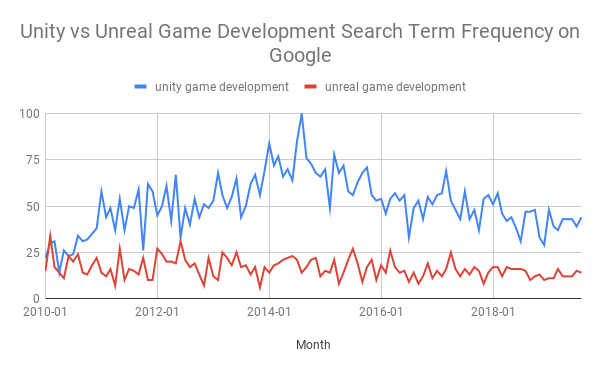
\includegraphics[width=6in]{images/googletrends-unity-game-dev-vs-unreal}
	\caption[Unity vs Unreal Search Term Frequency]{A graph from Google Trends showing the search term frequency of "unity game development" versus "unreal game engine development" from 2010 (Marking the release of version 3 of Unity). The vertical axis represents the percentage of popularity.}
	\label{fig:googletrends-unity-game-dev-vs-unreal}
\end{figure}

\filbreak
Unity3D is a game engine for creating interactive media. Launched in 2005, the goal was to create an affordable system for amateur game developers.\cite{unityHistory} By focusing on a simple asset pipeline and workflow, Unity3D thrived and by 2010 had over 200,000 registered users. Quickly, Unity became the \#1 platform for game development. \cite{unity3ReleaseNews}

The major competition to Unity3D is the Unreal Engine. Initially developed by Tim Sweeney, this engine was designed to push the limits of graphics and realism. Not only has it received a 2014 Guinness World Record for "Most Successful Game Engine", but also a long list from game developers and film productions alike.\cite{unrealAwards} However as shown in Figure \ref{fig:googletrends-unity-game-dev-vs-unreal}, Unity3D is more searched on Google for game development topics supporting the notion that it is the preferred tool for most games. 

A Bachelor's thesis written by Simo Ahola describes the steps necessary to build a Virtual Reality application in the Unity3D game engine supporting two different headsets: the HTC Vive and Oculus GO. By just downloading the individual SDKs then dragging and dropping the associated prefabricated component, Simo had easily developed a VR application.\cite{aholaUnityVR} 

It is of my personal desire to make CAVE development as simple and accessible as a headset. Unity's history of simplicity has positioned it in the forefront of VR development, making it the preferred platform for the vDen. 


\filbreak
\Section[Unity SDK]{Unity SDK}\label{sec:unitySDKSection} \\

The simple act of downloading an SDK and dragging the necessary components into your scene sounds so fundamental, however it was not until WYSIWYG game engines became popular for this to happen. The architecture of the vDen SDK revolves around this concept.

To guide development, we defined three goals for our system: rendering immediately upon importing, allowing full extension and of peripherals, and lastly simulating the vDen rendering in Unity itself.

The core rendering system govern the functionality of the eye and display cameras.

\noindent\textbf{Eye Cameras} \\

\begin{figure}[H]
	\centering
	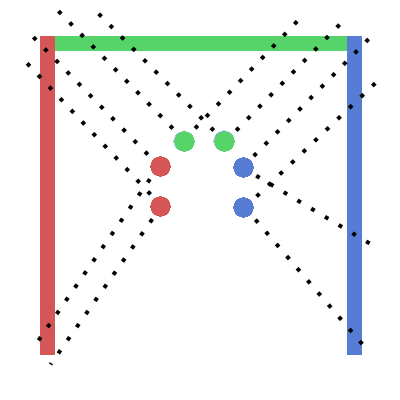
\includegraphics[width=3in]{images/camera-pairs}
	\caption[The Pairing of Eye Cameras]{The Eye Cameras are paired together and are related to a specific screen. Each camera pair has space in-between related to the inter-pupillary distance of the user's head. The floor cameras are missing in the graphic, but are in the SDK, bringing the total to 8 eye cameras.}
	\label{fig:eye-camera-pairing}
\end{figure}

Eye cameras capture an image that represents the view from a user's physical eye. As shown in Figure \ref{fig:eye-camera-pairing}, there are two cameras per screen, totaling 8 in the SDK. A pair of cameras are spaced apart along the shared axis with the distance equivalent to the user's interpupillary distance. Futhermore, each pair needs to remain orthogonal to the others. Lastly, because the screens represent a window to the world, we need to calculate a custom frustum for each camera.

\begin{figure}[H]
	\centering
	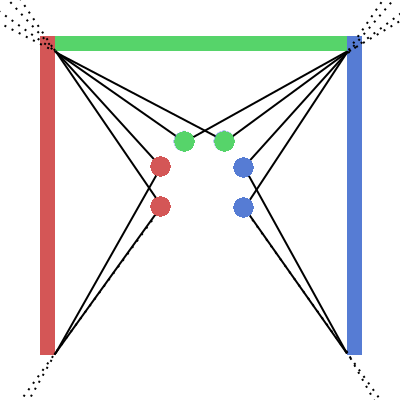
\includegraphics[width=3in]{images/camera-pairs-calibrated}
	\caption[The New Frustum of Eye Cameras]{Shows the new frustum of each camera after calculation. This provides the correct view as our physical screens represent windows into the world}
	\label{fig:eye-camera-frustum}
\end{figure}

Looking at the differences between Figure \ref{fig:eye-camera-pairing} and Figure \ref{fig:eye-camera-frustum}, we can immediately see the frustum is bounded to the the screen. This bounding guarantees that nothing is rendered outside of the screens. 

--- FIXME ---
The calcuation of a new frustum is easy. We need to determine the

\filbreak
\noindent\textbf{Display Cameras} \\
Display Cameras will output the final image for the projectors. With one camera per projector, the vDen has four total. The camera is associated with a pair of eye cameras and is responsible for merging their output together, left-right or top-bottom, for sterescopy, then rendering on the calibration mesh.

\filbreak
\noindent\textbf{Head Tracking} \\
A core feature of Virtual Reality is the generation of perspective correct imagery. This is done by understanding the head position and how the eyes view the scene. In order to track the head, the user dons a trackable baseball cap the tracking system syncs its position with the collection of eye cameras.

\Section[Dashboard]{Dashboard}\label{sec:dashboardSection} \\

\clearpage

\Chapter{Discussion}\label{chapter:discussionChapter}



In 2011, led by Thomas DeFanti, a team of 25 researchers set out to enumerate the requirements of an ideal CAVE and showcase the systems that have been developed to try and achieve these goals 
\noindent\cite{defanti-future-cave}. They list the  requirements as 


\begin{table}[H]
	\centering
	\renewcommand\arraystretch{0.5}
	\begin{tabular}{l | l}
		Hardware Requirements &  Software Requirements\\ 
		\hline
		- Compact footprint &  High resolution \\ 
		- Scalability &  Highbrightness and contras\\ 
		- Usability &  Input and full recognition of the viewer’s or viewers’ being and actions \\ 
		- Low noise signature & Audio (sonification) at or exceeding human aural acuity,   \\ 
		- Low thermal signature &  Touch (tactile) input and output\\ 
		- Holds several users  & No user encumbrances (special glasses, headphones, nose tubes)\\ 
		- Network connected & Olfactory (smell) output delivered to each user, \\ 
		- Extended service intervals &  Taste output and input recognition \\
		- easy access for maintenance &  Linking such devices together with near-zero latency\\ 
		- Power-efficient &  \\ 
		- Articulated, easily shippable screens &  \\ 
		- rapid installation/de-installation &   \\ 	
		- low-cost  &   \\ 
	\end{tabular} 
	
	\label{tbl:defantirequirements}
	\caption{Enumerates all of the requirements DeFanti's team listed}
\end{table}

The systems presented by the DeFanti et Al try to maximize compliance with the software requirements and a looser authority on the hardware requirements. 

This thesis presented showcases a true CAVE system that fully conforms to the hardware specifications of DeFanti \cite{defanti-future-cave} but also provides additional requirements to emphasize the importance of a floor projector. 

The purpose of this system was to fill in the latest gap of research in Low Cost IPT systems  from 2010 with Dr. Carolina Cruz-Neira to today. The landscape of modern virtual reality has changed, the advent of game engines to ease development and the wave of affordable headsets brings new requirements for a CAVE.

This CAVE system attempted to fully minimize the cost of production by utilizing off the shelf components and freely available software. 


\clearpage

\Chapter{Conclusion}\label{chapter:conclusionChapter}


\clearpage


\bibliographystyle{ualr-dissertation-IEEEtran}
\bibliography{references} 


\end{document}  % end of document
